\documentclass{beamer}



\mode<presentation>
{
  \usetheme{Berkeley}
%	\usetheme{Berlin}
%   \usecolortheme{}
%   \useinnertheme{circles}
   
  \setbeamercovered{transparent}

}


\usepackage[english]{babel}
\usepackage[utf8]{inputenc}
\usepackage{times}
\usepackage[T1]{fontenc}
\usepackage{multimedia}
\usepackage[absolute,overlay]{textpos}
\usepackage{graphicx}

\usepackage{xcolor}
\usepackage{amsmath}
\usepackage[absolute,overlay]{textpos}

\graphicspath{{./media/images/}}

\definecolor{paint}{RGB}{150,0,0}
\setbeamercolor {structure} {fg=paint}
\setbeamercolor{title}{fg=black}
\setbeamertemplate{itemize items}[circle]


\title[Tuning the computational architecture for Quantum Espresso ab initio calculation of nanostructures] % (optional, use only with long paper titles)
{Tuning the computational architecture for Quantum Espresso ab initio calculation of nanostructures}

\author[Giorgio Ruffa] 
{Giorgio Ruffa}
\institute[Università degli Studi di Milano]{Università degli Studi di Milano}

\date{28 Aprile 2016} 

\subject{}


\begin{document}

% ********** 1 slide *****************
\begin{frame}
  \titlepage
\end{frame}

\section{Introduzione}

% ********** 2 slide *****************
\begin{frame}{Introduzione}
\begin{picture}(100,100)
	\put(0,100){
\includegraphics[width=3cm]{beam_qe_logo.jpg}}
\end{picture}

\begin{textblock*}{3cm}(7cm,2cm) % {block width} (coords)
	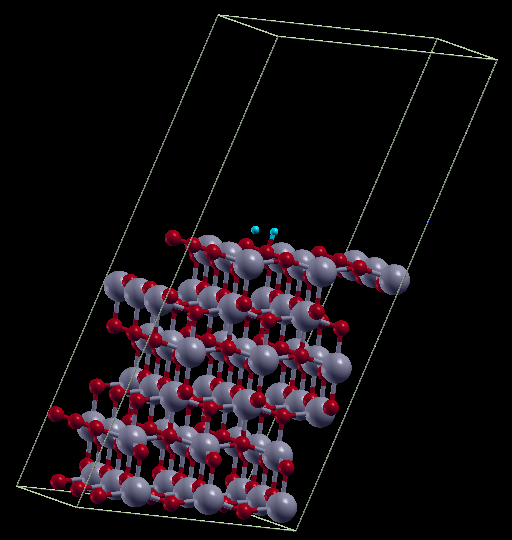
\includegraphics[width=3cm]{titania_crystal.png}
\end{textblock*}

\end{frame}



\end{document}